In this section, we describe the tracking experiment and all the tecquiques involved.

\subsection{Aim of the Experiment}

The focus of the last part of the Project is to track continuously two vehicles that are moving in a straight line,
and in particular to appreciate the advantages that the LMS beamformer in Frequency domain can offer.

\subsection{Geometry and Paramters}
The two vehicles are moving one towards Nord and one towards Est at 60 $km/h$. The antenna is placed in the origin at a height of 25 meters
and it is equipped with an array of 16x16 Antennas parallel to the ground. The simulation lasts 12 seconds and each vehicle 
exchange 24 packets in total.

This is the Scenario:

\begin{figure}[ht]
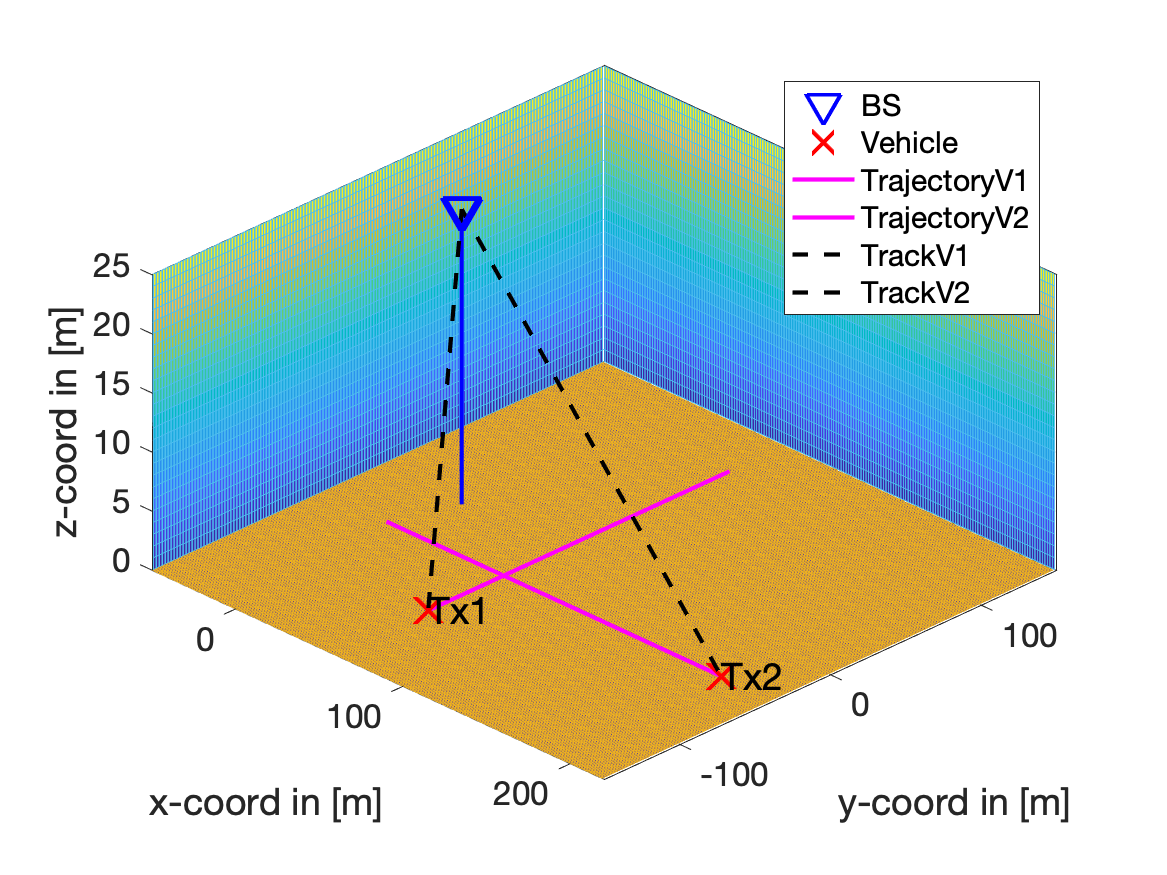
\includegraphics[width=\linewidth]{Quadriga1.png}
  \caption{Scenario.}
  \label{fig:Scenario}
\end{figure}

As parameters we used Carrier Frequency fc = 2.6 $GHz$, OFDM with 4-QAM as modulation with 64 sub-carrier and 100 symbols/packet.

\subsection{Steps of the Simulation}

\begin{enumerate}
    \item \textbf{Generation of the signals} Through the QAM modulator and OFDM modulator. 
    \item \textbf{Creation of the Channel} In this case $QuaDRiGa\_UD2D\_LOS$ channel.
    \item \textbf{Passage of Waveforms in the channel} By means of the convolution with the channel model.
    \item \textbf{Estimation of DoA} With the Music Algorithm.
    \item \textbf{OFDM Demodulation} Applying the FFT on the Signal from each Antenna.
    \item \textbf{LMS Beamformer} For each sub-carrier (In Frequency Domain) using half of the sequence as training.
    \item \textbf{Channel equalization} Applying the Gradient-Descent algorithm to each Sub-Carrier.
    \item \textbf{QAM Demodulation} Finally recovery of the bits and calculation of the BER.
\end{enumerate}


\subsection{Results of the Tracking}

The experiment shows that at the beginning the Tx with Vehicle1 has practically zero errors since it is the nearest to the station
and the music algorithm can estimate without problems its position. Instead the Tx with Vehicle2 has many more errors, due to 
the many multipath of the channel and to the lower received Power (Figure \ref{fig:Begin_tx}).

When they are about the same distance and in normal conditions the track performs without any particular problem (Figure \ref{fig:Middle_tx}).

At the end when Vehicle2 is the nearest to the BaseStation, the situation is inverted and the Tx with Vehicle2 is far more 
reliable that with Vehicle1 (Figure \ref{fig:End_tx}).

\begin{figure}[ht]
    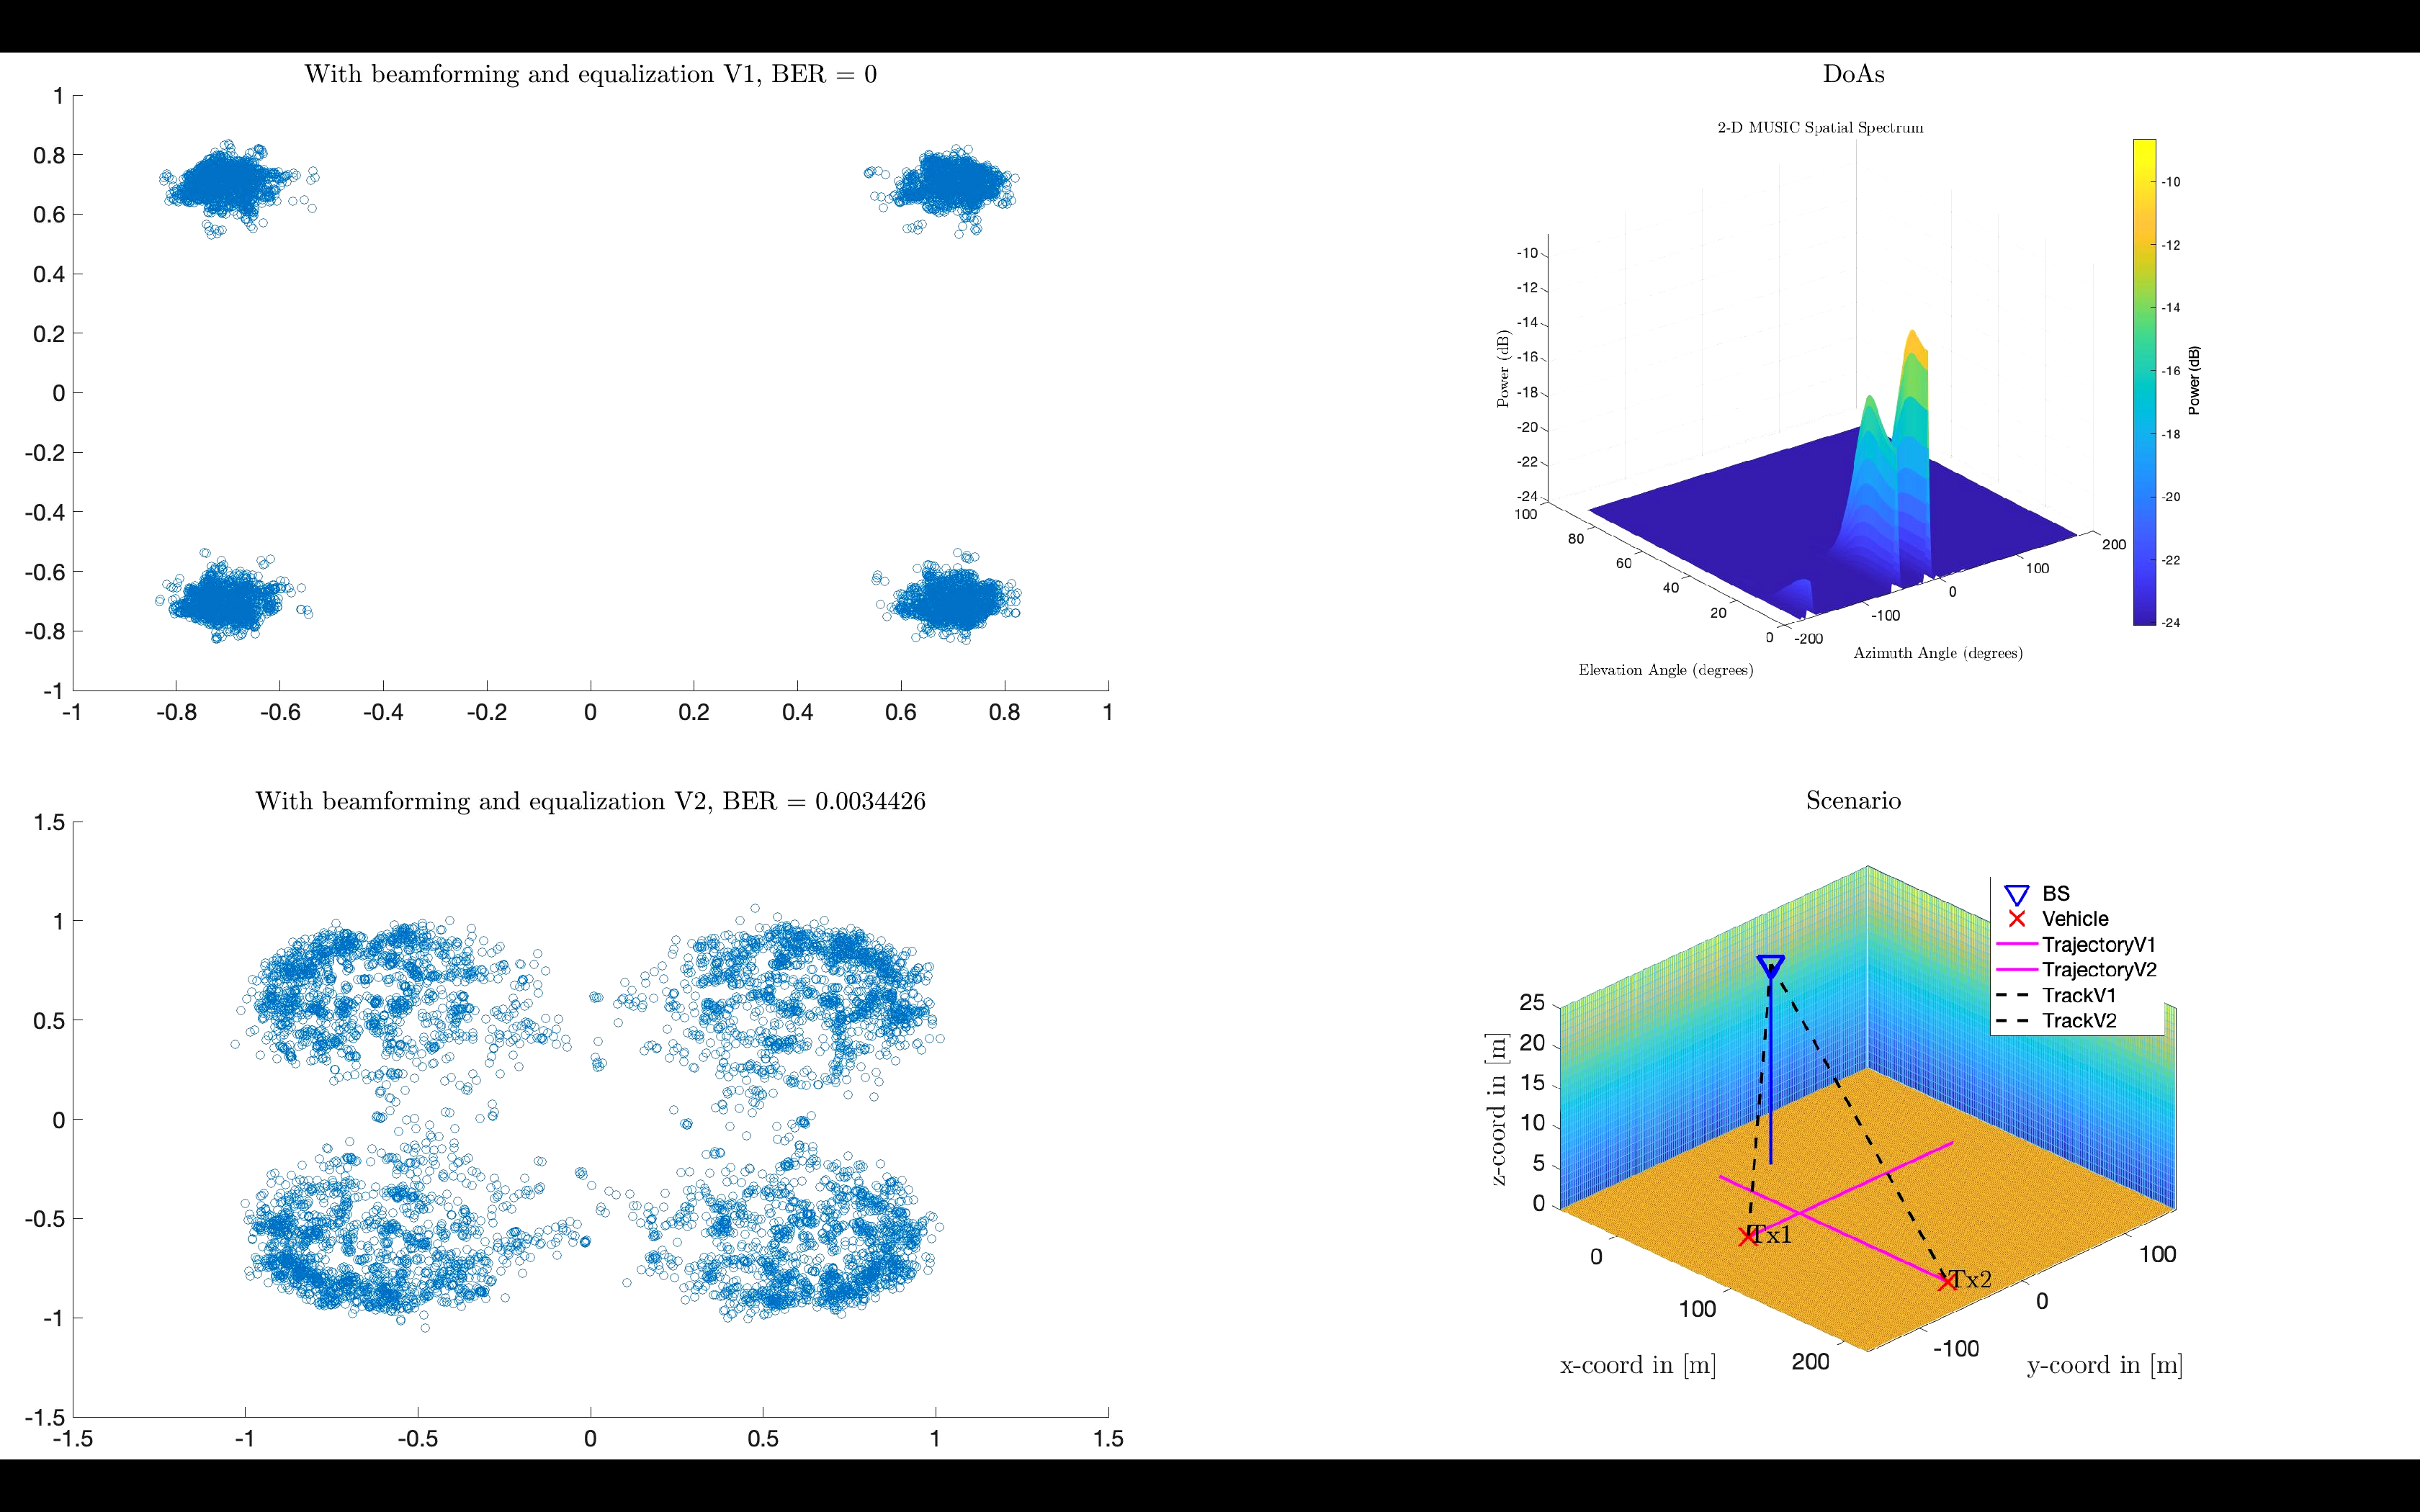
\includegraphics[width=\linewidth]{Begin_tx.png}
      \caption{Beginning of Tx.}
      \label{fig:Begin_tx}
\end{figure}
\begin{figure}[ht]
    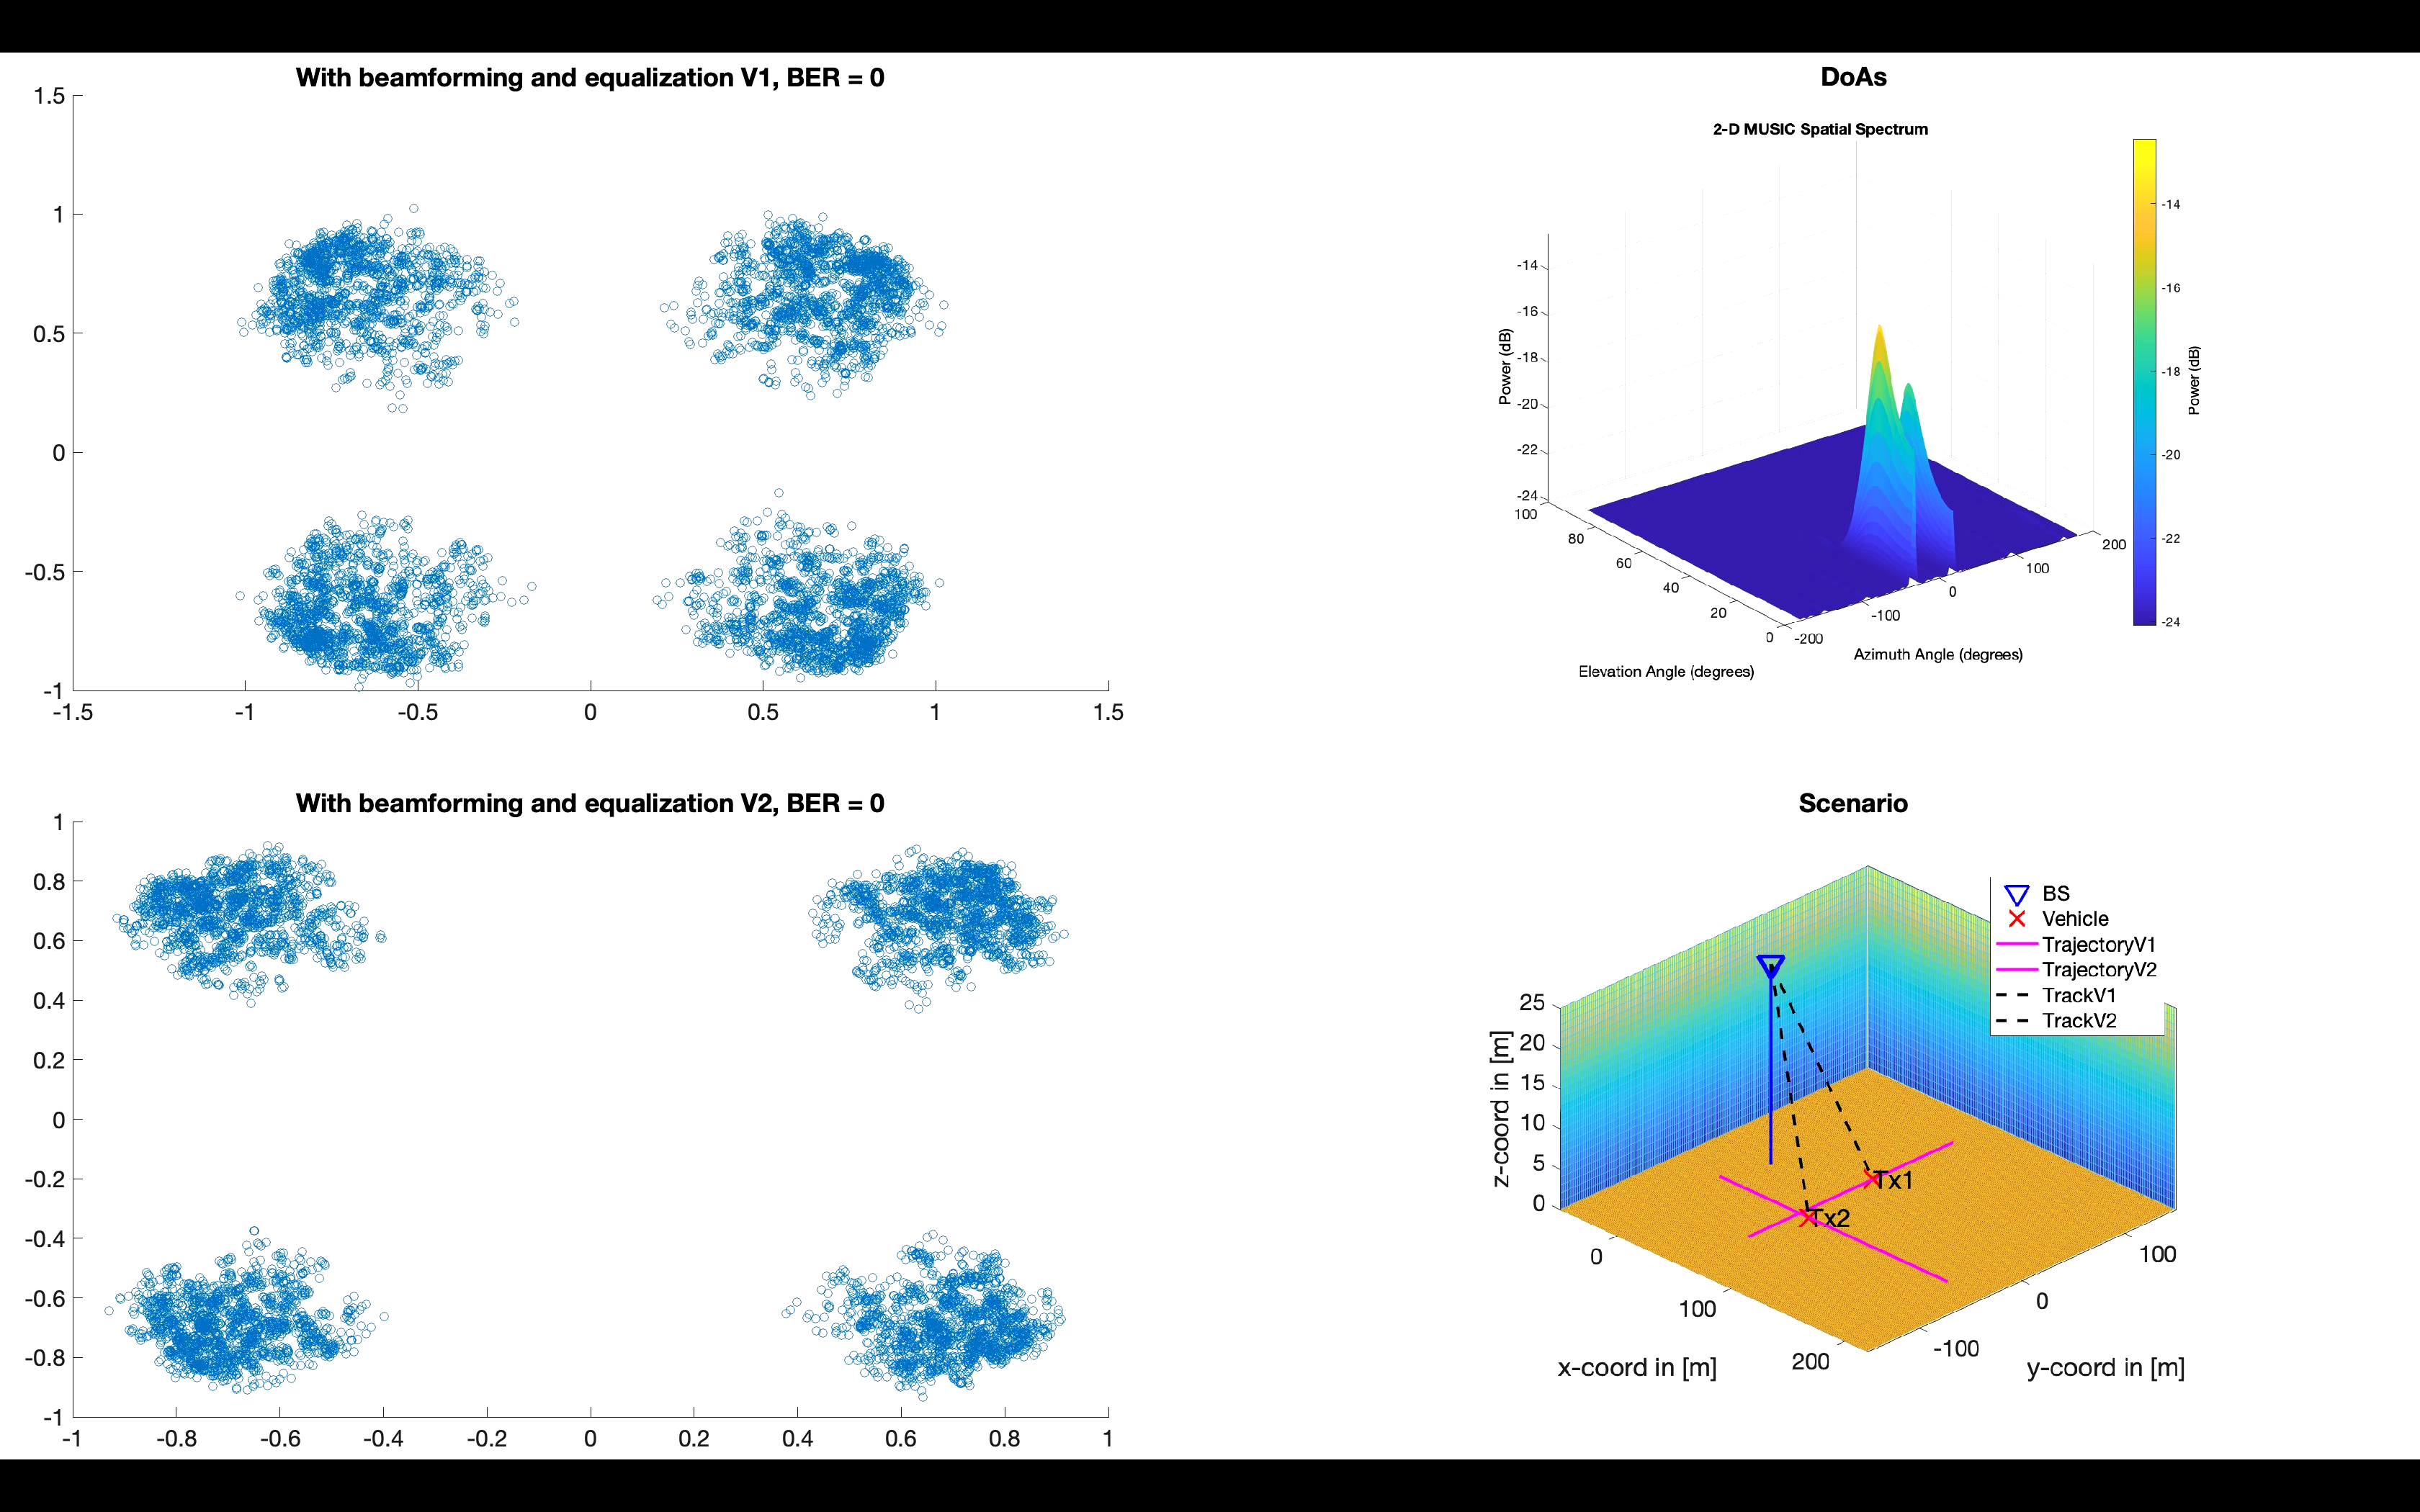
\includegraphics[width=\linewidth]{Middle_tx.png}
      \caption{Middle of Tx.}
      \label{fig:Middle_tx}
\end{figure}
\begin{figure}[ht]
    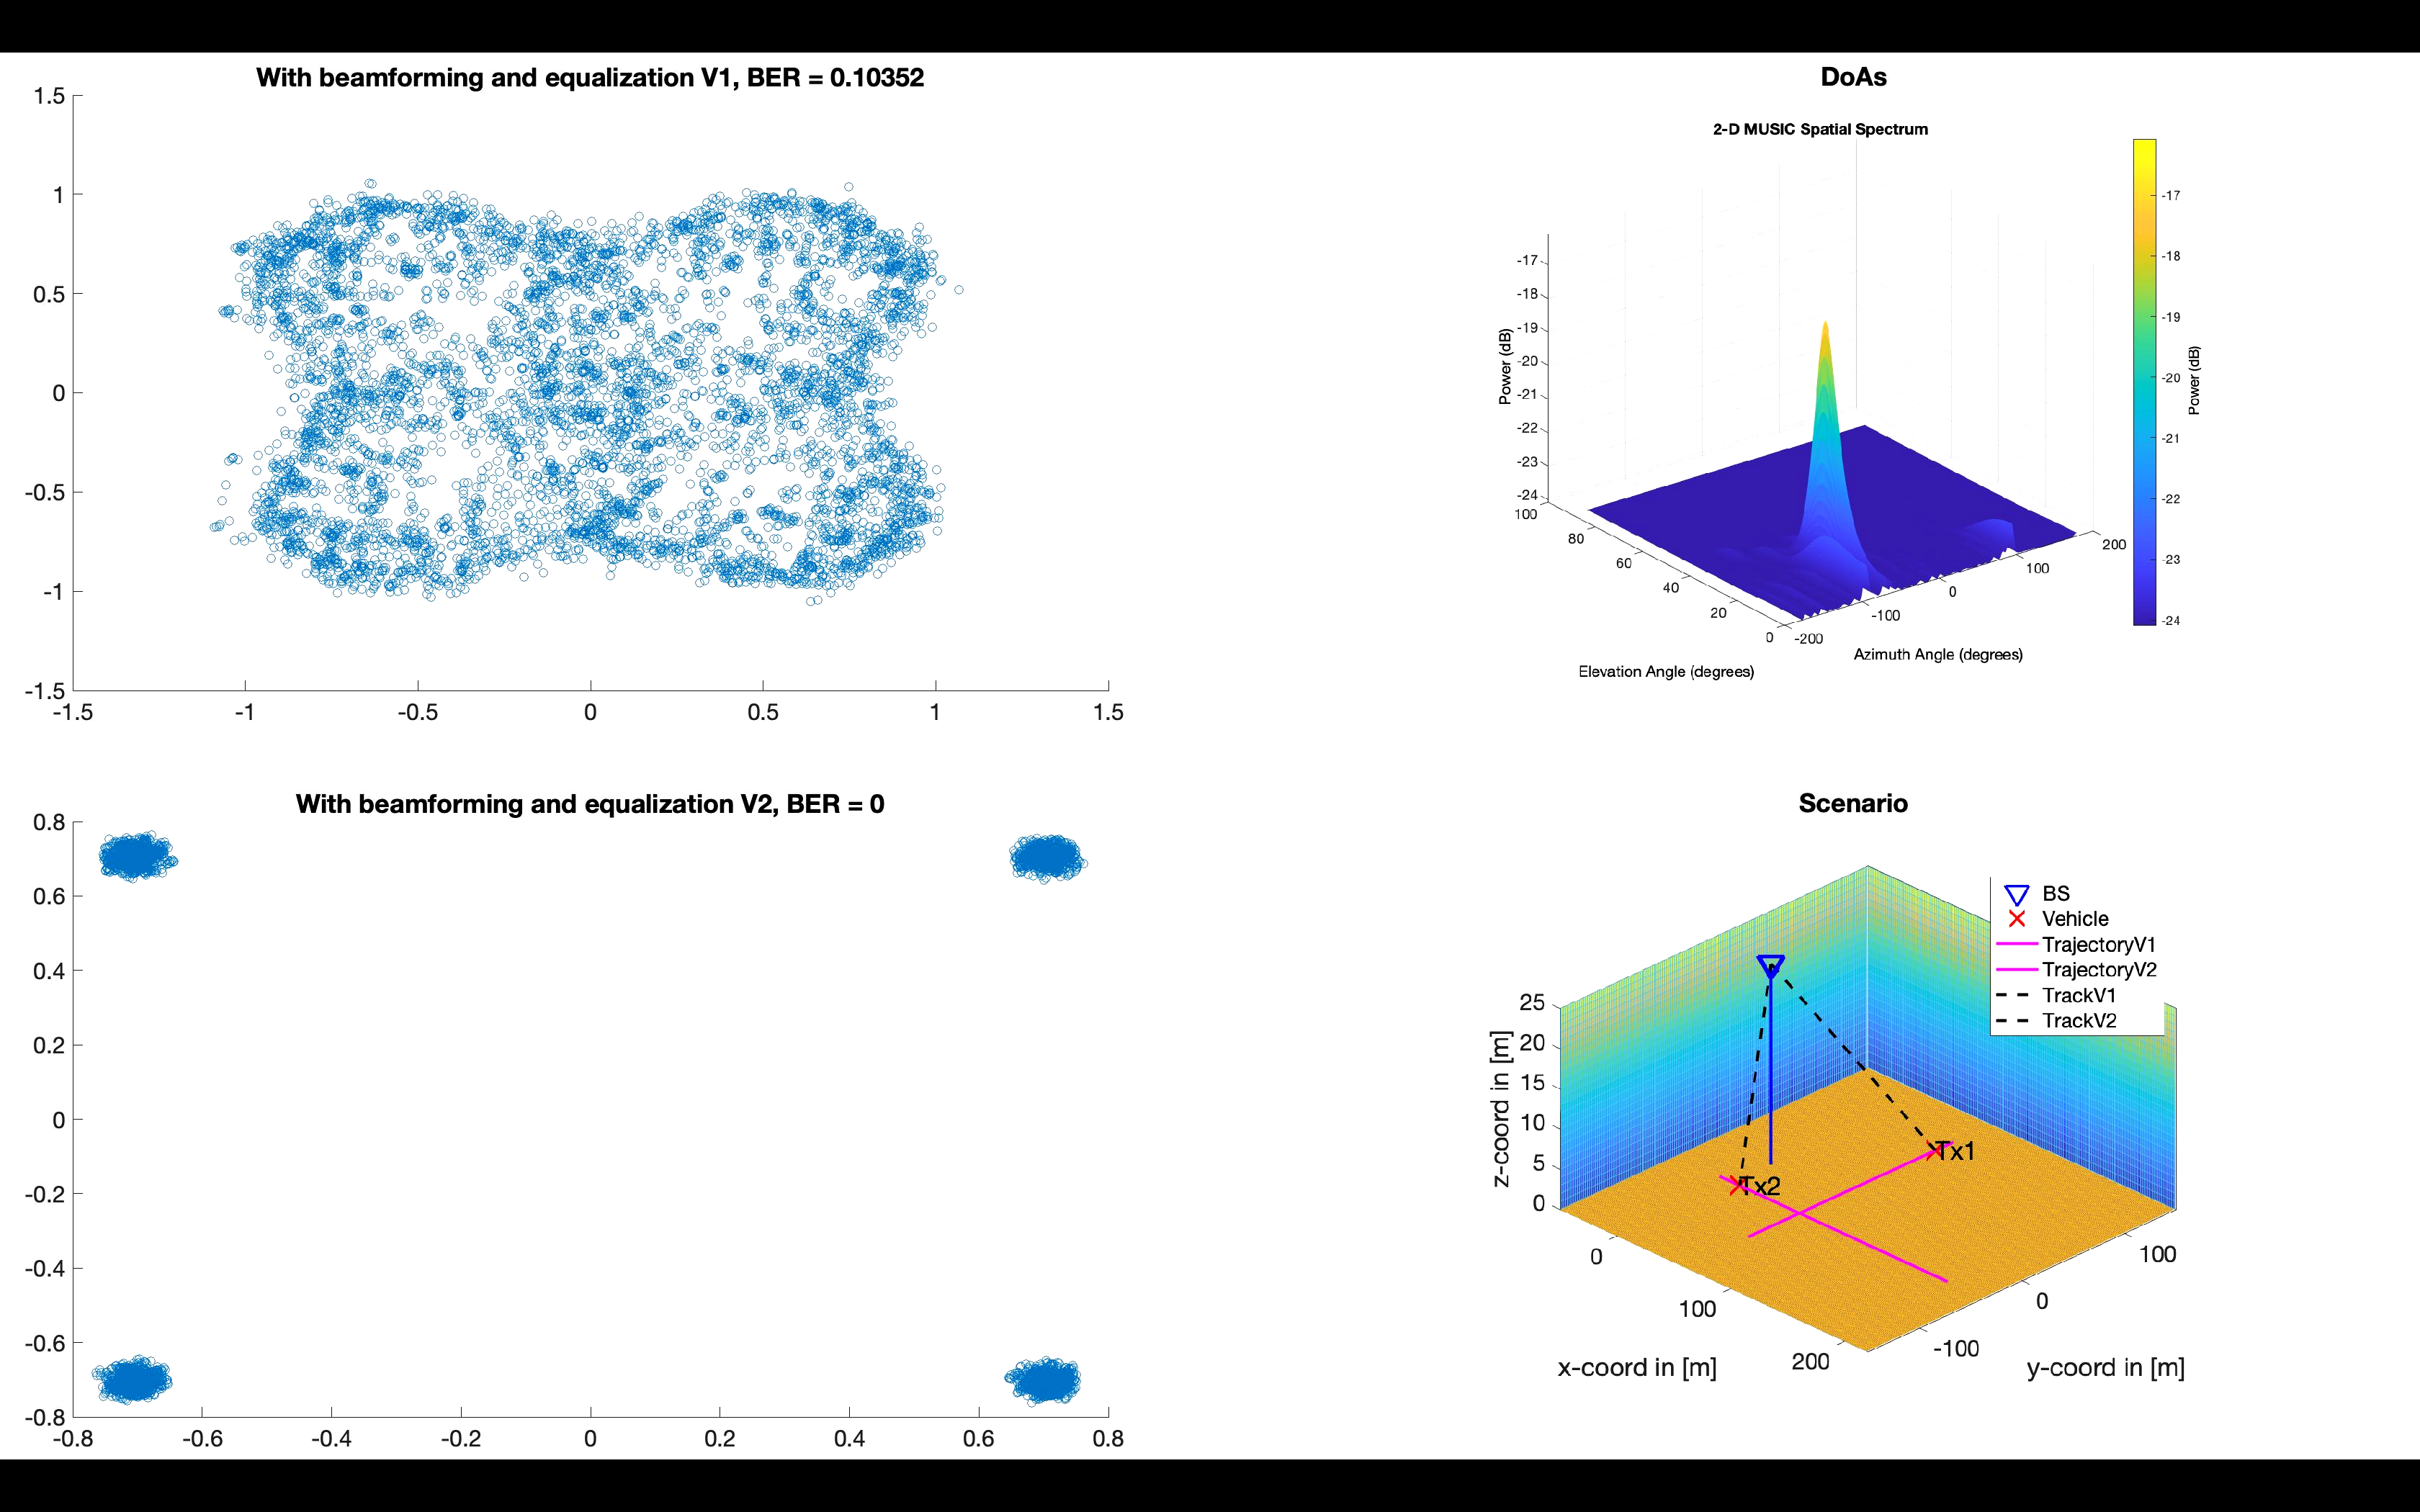
\includegraphics[width=\linewidth]{End_tx.png}
      \caption{End of Tx.}
      \label{fig:End_tx}
\end{figure}
